\documentclass{article}
\usepackage[utf8]{inputenc}
\usepackage[margin=1in]{geometry}
\usepackage{graphicx}
\usepackage{url}
\graphicspath{{./images/}}
\usepackage{xcolor}
\usepackage{amsmath}
\usepackage{listings}
\usepackage[english]{babel}
\usepackage{enumerate}
\lstset{frame=tlrb,xleftmargin=\fboxsep,xrightmargin=-\fboxsep}
 
\usepackage[style=numeric, backend=biber, maxcitenames=2]{biblatex}
\bibliography{bib/references}

 
\begin{document}

\title{Population Synthesis Literature Review}
\author{Jin Zhou}
\maketitle


\section{Goal}
Since the step of urban typology has been done, we need to fill in the blank between city clustering results and a complete SimMobility\cite{adnan2016simmobility} input of virtual city.
The city model that SimMobility takes as input has two components.
One is the demand and the other is the supply, which includes the road and transit network.
To model the demand, a methodology has to be developed to construct the population with desired demographics and allocate the population in space.
Next to it, we also need to figure out how to use the synthesized households and individuals in disaggregate level to get the travel demand in the city.
The literature review at this time is to gain a better idea of previous efforts to address the problem of population synthesis and assignment. 

\subsection{Questions:}
\begin{enumerate}
	\item What should the input of travel demand generation look like? This guides the adaptation of population synthesis method from literature.
	\item What attributes should be included to characterize the population? Age, sex, educational level, and there must be some attributes reflect the traveling behavior of people. 
	\item Do we synthesize households or personnel? Or how to match individuals to households?
	\item We need to come up with a solution to cities don't have PUMS data and virtual cities that don't even have census data for demographics.	
\end{enumerate}


\section{Prior Work}

Household assignment and spatial allocation are two big issues we need to solve when facing the problem of population synthesis.
Specifically, the first one addresses the problem of how to match individuals to the household where they belong, while the spatial allocation distributes households in geographical space.
It is necessary because the ultimate goal of our work is to do transportation simulation, which can only be achieved by knowing the location of each agent. \\

There has been lots of literature on population synthesis.
The methods used varies from Iterative Proportional Fitting (IPF), MCMC-based sampling \cite{farooq2013simulation}, to Bayesian network approach \cite{sun2015bayesian}. The original work in this field is presented in \cite{beckman1996creating}. It used a method called Iterative Proportional Fitting (IPF) to synthesize population based on data from two sources. What they do is iteratively fitting the cells of a multi-way contingency table expanded by attributes that characterize a household/individual so that it satisfies the constraints of marginal distribution of demographics and also preserves the correlation structure carried by sample data of the whole population. Here the marginals of demographics comes from census data in the level of census tract or block group while the correlation structure need to be derived from survey data of target population. In case of the absence of disaggregated sample data, IPF can still give a solution by iteratively adjust the cells in accordance only with the marginal constraints. However, lots of different joint distributions can share the same marginals and IPF may converge to anyone of them. This is certainly a downside of traditional IPF, and is also the reason why we need the correlation structure of sample data to make the solution captures the true population distribution. After the fitting of the table, a desired number of synthetic population is sampled according to individual or household weights in the table. And this is where the sensitivity of IPF to the quality of data and the sample size stems from. In this method, spatial allocation is solved concurrently with the population synthesis, since it generates the population for each zone and then adds up to the whole population. On contrary to this, one can also synthesize the total population first and then allocate them to different zones. However, this includes implementing a detailed matching method between households and zones, like what's developed in \cite{ge2014virtual}, which is also very time-consuming. 

Ever since Beckham et al. used IPF to do population synthesis, limitation of this method and the targeted modification has been published by other researchers. By IPF alone, one can only separately generate a set of weights either for individual or household. According to \cite{ye2009methodology}, the synthetic population generated based on the application of household weights can give a joint distribution of person attributes far from the given person marginal distribution.
This is due to the fact that all persons are just simply selected from chosen households according to household weights.
\textcite{ye2009methodology} has improved this problem of IPF by a method called Iterative Proportional Updating (IPU), and they claim that the algorithm they proposed can match the person-level distribution and household-level attributes as closely as possible. \\

MCMC-based sampling is brought up by \textcite{farooq2013simulation}.
The problem is defined as how to use partial views, including samples and conditional distributions, to estimate the true joint distribution of population attributes, where the attributes are defined as $X = (X^1, X^2, ... X^n)$.
Here, they used Gibbs Sampling to generate certain amount of population based on prior knowledge of the joint distribution and proved that the sampled population is very much similar to the true simulation in the statistical sense.
It has been pointed out that, since the task of getting full conditionals won't be trivial in reality, they replaced some of conditional distributions by marginal distributions.
Thus, if one wants to implement MCMC, the sample data of the entire population is fundamental.
Furthermore, the derivation of conditional distribution is not trivial especially when the number of attributes gets large.

The population synthesis method that \textcite{petrik2016measuring} used adapted ideas from probabilistic graphical models (PGM).
In their graphical model, there are 7 socio-demographic attributes, which are Age, Gender, Employment, Income, Car ownership, Purpose of trip, and Who pay for the trip, to represent a person.
Once the dependencies between variables are specified, we need to calculate or estimate conditional probability of one node given its parents.
The flexibility of this method is that those conditional probabilities can be derived from different sources like census data or surveys on individuals. Nevertheless, compared to the high dependency of IPF on the quality of sample data, Bayesian method gives synthetic population more heterogeneity.
Finally, the synthetic population is just random draws from the probabilistic graphical model.
Though we can take marginal distributions of all variables as supplement for the graphical model, the population generated by Bayesian network model can only precisely match the marginals of mother nodes.
This is because the distribution of a node is uniquely defined by its parent node and the conditional distribution based on PGM.
And this point should be taken into consideration when choosing the population synthesis method. 


\section{Data}
Most paper in population synthesis used Public Use Microdata Sample (PUMS) data, which is available both in individual level and household level.
It includes multiple socio-economic parameters of a household or an individual in the region.
The sample rate of this dataset is about 1\% to 10\% of the total population in the region. 
PUMS data is very complete in US cities and can be easily downloaded from government census website \footnote{https://www.census.gov/programs-surveys/acs/data/pums.html}, but the same data for cities in developing countries can be relatively outdated and harder to find. The sample data is used as seeds to initialize the contingency table in IPF methods. Another important part of data is called aggregate data \footnote{https://factfinder.census.gov}. They give marginal distribution for variables of our interests. It's worth noticing that the marginal distributions for subsets with more than 2 variables can be rarely found. An ideal format for aggregate data is that we have the marginal distributions in the level of geographical zone cause IPF is carried out separately in each zone. So when downloading the aggregate data, one should first choose a geographic type in corresponding to the zones in the virtual city, then specify the variables or tables you want.

The choice of algorithm should be based both on the data we have and the appearance of the final result we want.
What is also important for us is the simplicity and novelty of methodology. We will start from a conventional IPF method using data from Houston city, then according to the execution time and the accuracy of the result we will make further extension to IPF method.


\section{Iterative Proportional Fitting}

Using IPF to synthesize population includes two major steps.
In the first step, the disaggregate samples of population are used to initialize the contingency table expanded by attributes, and the fitting is carried out to meet marginal constraints from aggregated data.
In the next step, the fitted contingency table is used to sample the population.
To describe IPF, we need to define the contingency table it fits.
Suppose a person or household is described by \textit{m} attributes (or demographics), then we need to develop a m-way table.
For each demographic $i$, there are $n_i$ categories.
Thus, a cell $(i_1, i_2,..., i_m)$ represents a kind of person/household, where $i_j = 1,2,...n_j$ is the observed value of the $j$-th demographic with $n_j$ categories it can choose from.
From sample data like PUMS, $n$ is the total number of observations while $n_{i_1, i_2,...,i_m}$ is the counts for people/household of this type.
Hence, the proportion of this type in the sample is denoted by
\begin{equation}
  \label{eqn:prop}
   p_{i_1,i_2,...,i_m} = \frac{n_{i_1, i_2,...,i_m}}{n}
\end{equation}
The constraints is defined as $T_k^j$, which is the marginal totals for the $k$-th category of attribute $i$ from census data.
We can easily get the equation
\begin{equation}
  \label{eq:2}
\sum_i\sum_{k=1}^{n_i}T_k^j=n.  
\end{equation}
Let $p_{i_1,i_2,...,i_m}^{(t)}$ denote estimated proportion of cell $(i_1, i_2,..., i_m)$ in iteration $t$ and
\begin{equation}
  \label{eq:3}
  p_{...,i_j=k,...} = \sum_{i_1=1}^{n_1}...\sum_{i_m=1}^{n_m}p_{i_1,i_2,...,i_j=k,...,i_m}^{(t)}  
\end{equation}

The IPF starts with initiating all weights in the contingency table by  
\begin{equation}
	p_{i_1,i_2,...,i_m}^{(0)} = p_{i_1,i_2,...,i_m}
\end{equation}
and in each iteration, the proportions are updated by the formula
\begin{equation}
  p_{i_1,i_2,...,i_j=k,...,i_m}^{(new)} = p_{i_1,i_2,...,i_j=k,...,i_m}^{(old)} * \frac{T_k^j * p_{...,i_j=k,...}^{(new)}}{n} 
\end{equation} for all categories of each attribute, until it converges.
Within an iteration, $p^{(old)}$ for the first marginal corresponds to $p^{(t-1)}$, which is the result from last iteration.
And for marginals come next, $p^{(old)}$ should be set to proportions calculated from previous marginals.
According to \cite{beckman1996creating}, the algorithm converges in 10 to 20 iterations.

In the next step, the synthetic population shall be constructed by selecting households from PUMS in proportion to the estimated weights in the multiway table. Or we can do Monte Carlo sampling method to draw households from estimated weights from IPF.
Specifically, the number of households of each demographic type in a census tract can be obtained by multiplying the total number of households by the probability in the cell representing this household type, or by drawing the numbers at random according to these probabilities.
However, the household type represent by a cell in multiway table is not exactly that of PUMS data.
The fitted multiway table can only be span by control variables, which is defined as variables which have marginal distribution in census data.
However, households and individuals in disaggregate data are usually described by additional desired variables.
So, the probability of a household type in PUMS data being chosen shall be assigned according to the distance between such a household $p$ and a household type $c$ in multi-way table.
In \cite{beckman1996creating}, this probability is defined as 
\begin{equation}
	D(p,c) = w_p \prod_{i \in J}\Big(1-|(d_i^p-d_i^c)/r_i|^k\Big)*\prod_{i \notin J}\Big(1-\Delta(d_i^p, d_i^c)\Big)
\end{equation}

\section{Proposed method}

\begin{enumerate}[Step 1:]
\item Network: modify OSM network file, make it legal input to SimMobility
  \begin{enumerate}[1.]
  \item links has to be unidirectional
  \item shorten the links and add turning points
  \item maintain the attributes of each object in the network
  \end{enumerate}
\item Population Synthesis
  \begin{enumerate}[1.]
  \item Data collection: sample data, aggregate data for zones in each city
  \item Data processing: categorize sample data and get joint distribution, formatting aggregate data
  \item Apply IPF algorithm and use the weights result to draw synthetic population
  \item Assign households in each county to locations based on land use information
  \end{enumerate} 
\end{enumerate}

Although applying IPF to population synthesis is prevailing and the idea is straightforward, the algorithm itself is time consuming and expansive once the combinations of demographics gets large.
Suppose we have 2 gender categories, 7 age groups, 5 income groups, 5 levels of education, 9 types of occupation, 2 kinds of car ownership, and 5 household types.
These alone give rise to $31\,500$ types of individuals, not to mention describing individuals with more demographics.
Another issue with published methods is that the time we spend to generate population for one zone has to be multiplied by the number of zones in a city in order to get the whole population for the city, which means the time for a complete process is hundreds of that for a single zone if the zone is in the sense of census tract.
Since what we want is something less time consuming, a new methodology has to be developed.

Considering the accessibility of the two sources of data that the synthesizer needs, one can always get sampled survey data in a city level but not necessarily census data for zones in a city.
Given the global scope of our problem, there are cities whose zones are even not defined properly.
Thus, we will face the problem of defining the zones of a city by our own in case of the data is in shortage.
In developing the zones in a city, we will borrow the idea of zones from \textcite{fielbaum2016parametric}, where a city is divided into one CBD and subcenters along with their peripheral.
It has to be admitted that in this way, we will not have aggregate census data for zones. This is a problem we will address later. 

\subsection{Data processing and IPF}
In detail, the data processing and IPF includes following steps: Getting marginal distribution of variables that we are interested in from Census Bureau; Processing the data of marginal distributions to convenient format; Getting sample data from PUMS, and selecting sample data in our metro area by mapping census tract to county; Selecting variables in sample data, categorizing sample data based on "PUMS codebook" and variables categories in aggregate data; Generating joint distribution of sample data, which means get the frequency of each kind of combination of characteristics in sample data; Using joint distribution of sample data and marginal distribution as input to IPF; Performing IPF algorithm; Using output joint distribution of IPF to draw synthetic population. 

\begin{figure}[h]
	\centering
	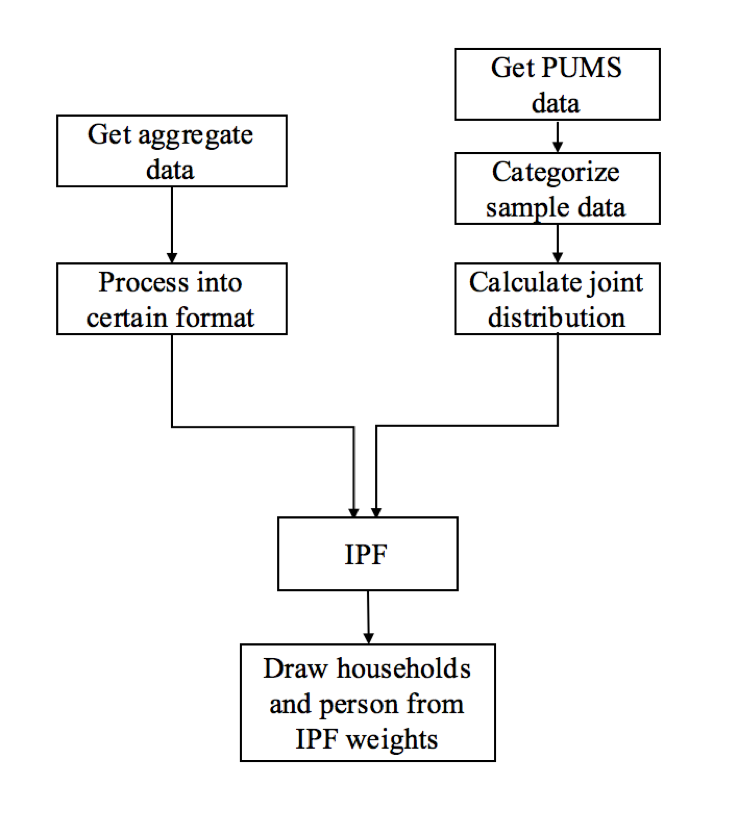
\includegraphics[width = 0.5\textwidth]{ipf_flow_chart.png}
	\caption{Flow chart of data processing and IPF}
	\label{fig: flowchart}
\end{figure}

In our first exploration, we have used 5 attributes to describe a households and they are household type, household size, household income in the last 12 months, number of vehicles and number of workers in the household. We not only find one dimensional marginal distribution for those variables but also two dimensional marginal distributions for household type $\times$ household size, number of workers $\times$ household size as well as number of vehicles $\times$ number of workers in the household. Across the process of data retrieving and processing, we find the categories each variable can have is largely depends on the availability and format of aggregate data.




\subsection{Two approaches to spatial assignment of households}
\subsubsection{K-means clustering}
With regard to the assignment of populations to zones, we will cluster the population at city level with K-means first.
We reason that similar and highly correlated people will most likely live in the same area within a city.
Then we obtain grouped people with similar attributes.
We choose K-means because it is more intuitive if we want a spatial allocation and the feature of hidden centroid for each cluster will hopefully capture the characteristic of the zone.

\subsubsection{Zonal disaggregation and random sampling}
\textcite{moekel2003microsimulation} present an intuitive approach to assigning households to zones, which we propose to implement.
First, they obtain land-use data, which they use to disaggregate zonal characteristics (e.g.\ household location or firm location) into raster cells.
The size of these cells are chosen based on computational tractability and desired resolution.
Weights are then assigned to the cells based on the corresponding land-use category.
For the household example, \textcite{moekel2003microsimulation} aggregate land-use attributes into the following: high-density housing, low-density housing, industry and open space;
to which weights of 10, 5, 1 and 1 are assigned, respectively.
The weights are then normalized by zone, and households are randomly selected to populate each cell to fit each proportion.
The address of each household is assumed to be the centroid of each cell, which each associated with its parent zone.
The rasterization is performed by a so-called ``point-in-polygon'' algorithm.
This approach presents a fast way for household assignment, assuming prior zonal assignment is available.
The populations themselves can first be generated using a simple IPF/U routine.

\newpage
\section{References}
\printbibliography[heading=none]
\end{document}
